\documentclass{article}
\usepackage{graphicx}
\usepackage{alltt}
\usepackage{amsmath}
\usepackage{amsfonts}
\usepackage{bigstrut}
\usepackage{enumerate}
\usepackage{fancyhdr}
\usepackage[top=1.0in, bottom=1.5in, left=0.75in, right=0.75in]{geometry}
\usepackage{float}
\usepackage{lastpage}
\usepackage{tikz}
\usepackage[latin1]{inputenc}
\usepackage{color}
\usepackage{array}
\usepackage{longtable}
\usepackage{calc}
\usepackage{multirow}
\usepackage{hhline}
\usepackage{ifthen}
\usepackage{listings}
\usepackage{circuitikz}
\usepackage{caption}
\definecolor{mygreen}{rgb}{0,0.6,0}
\definecolor{mygray}{rgb}{0.5,0.5,0.5}
\definecolor{mymauve}{rgb}{0.58,0,0.82}
\lstset{ %
  backgroundcolor=\color{white},   % choose the background color; you must add \usepackage{color} or \usepackage{xcolor}; should come as last argument
  basicstyle=\normalsize,        % the size of the fonts that are used for the code
  breakatwhitespace=false,         % sets if automatic breaks should only happen at whitespace
  breaklines=true,                 % sets automatic line breaking
  captionpos=b,                    % sets the caption-position to bottom
  commentstyle=\color{mygreen},    % comment style
  deletekeywords={...},            % if you want to delete keywords from the given language
  escapeinside={\%*}{*)},          % if you want to add LaTeX within your code
  extendedchars=true,              % lets you use non-ASCII characters; for 8-bits encodings only, does not work with UTF-8
  frame=single,	                   % adds a frame around the code
  keepspaces=true,                 % keeps spaces in text, useful for keeping indentation of code (possibly needs columns=flexible)
  keywordstyle=\color{blue},       % keyword style
  language=python,                  % the language of the code
  morekeywords={*,...},            % if you want to add more keywords to the set
  numbers=left,                    % where to put the line-numbers; possible values are (none, left, right)
  numbersep=5pt,                   % how far the line-numbers are from the code
  numberstyle=\tiny\color{mygray}, % the style that is used for the line-numbers
  rulecolor=\color{black},         % if not set, the frame-color may be changed on line-breaks within not-black text (e.g. comments (green here))
  showspaces=false,                % show spaces everywhere adding particular underscores; it overrides 'showstringspaces'
  showstringspaces=false,          % underline spaces within strings only
  showtabs=false,                  % show tabs within strings adding particular underscores
  stepnumber=2,                    % the step between two line-numbers. If it's 1, each line will be numbered
  stringstyle=\color{mymauve},     % string literal style
  tabsize=2,	                   % sets default tabsize to 2 spaces
  title=\lstname                   % show the filename of files included with \lstinputlisting; also try caption instead of title
}
\floatstyle{boxed}
\floatstyle{plain}
\restylefloat{figure}
\pagestyle{fancy}
\fancyhead{}
\fancyfoot{}
\setlength{\headheight}{59.0pt}
\def\inputGnumericTable{}
\fancyhead[CO]{}
\lhead{\today}
\rhead{Page \thepage{} of \pageref{LastPage} }
\newlength\tindent
\setlength{\tindent}{\parindent}
\setlength{\parindent}{0pt}
\renewcommand{\indent}{\hspace*{\tindent}}

\usepackage[toc,page]{appendix}
\usepackage{titling}
\setlength{\droptitle}{-3.5cm}

\title{Air Force Institute of Technology \\ Department of Electrical and Computer Engineering}
\author{CSCE 654 - Computer Communication Networks \\ Project \#4 - Network Routing \\ \\ Authors:  Micah Hayden, Lucas Mireles, Ryan Wilkerson }
\date{\today}

\begin{document}
\maketitle
%\begin{abstract}
%This is my abstract.
%\end{abstract}
\vspace{-1cm}
\section{Optimization Process/Methodology:}
We optimized our network using the following methodology.
Due to full-duplex communications, both directions of each link see the full link capacity.
Thus, for any pair of bases $A$ and $B$, we only need to optimize for the highest load of $\lambda_{A \rightarrow B}$ or $\lambda_{B \rightarrow A}$.

We thus minimized the score function by changing the configuration of links between each pair of bases, giving an optimal 4-connected topology.

After we had our optimal configuration, we removed the two lowest-loaded links to achieve 3-connectedness. 
This prevented as much additional strain on the existing infrastructure as possible.
We then optimized the remaining 8 links by routing the deleted channel's traffic through remaining channels.
The 3-connected topology had a better score by $\approx 0.3$.
This difference is small enough that the only way to know which network performs better is through simulation; thus, we are utilizing the 4-connected topology.

\section{Network Topology:}
\label{sec:Topology}

\begin{figure}[h!]
\centering
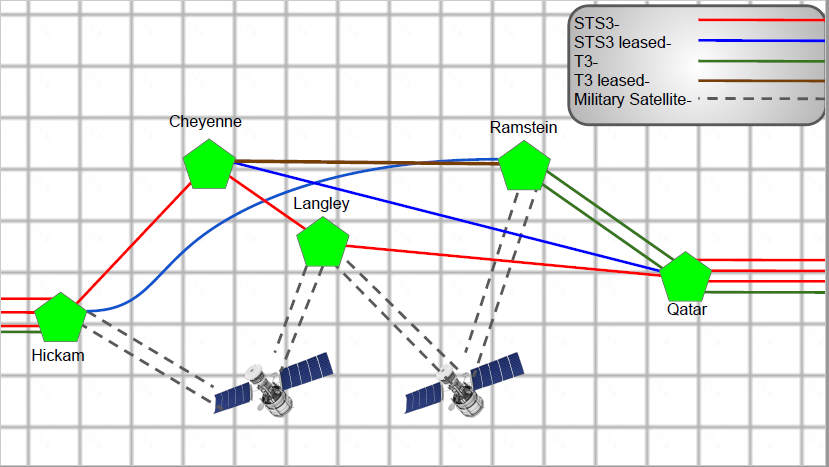
\includegraphics[scale=0.75]{Images/Topology.PNG}
\caption{Network Topology of Routing Network}
\label{fig:Topology}
\end{figure}

\newpage
\section{Cost Calculation:}
\label{sec:Cost}
Given the costs in the Project Requirements, we went through the following steps to build our total network cost.

\noindent \textbf{Installation Costs:} 

For any leased system, satellite or otherwise, there was no installation cost.
If there was an owned land line (STS-3 or T3), we incurred a trenching cost.
This cost is calculated as follows, where $d$ is the distance between the two nodes:
\begin{equation}
\text{Trenching Cost } = IC_{trench} = d_{A \rightarrow B} \cdot \text{\$}10,000
\end{equation}

For owned land lines, we incurred a per-link installation cost.
\begin{equation}
\text{Link Installation Cost } = IC_{link} = d_{A \rightarrow B} \cdot \frac{cost}{km}
\end{equation}

For any owned satellites (we have none), we would incur the following satellite installation cost, where $k$ is the cost of installing a given type of satellite:
\begin{equation}
\text{Satellite Installation Cost } =  IC_{sat} = k
\end{equation}

The overall installation cost is shown below:
\begin{equation}
\text{Installation Cost } = IC_{total} = IC_{trench} + IC_{sat} + \sum_{links} IC_{link} 
\end{equation}

\noindent \textbf{Monthly Costs:}

Each type of link had a given monthly cost, based on the type of link.
Additionally, each node communicating with a satellite has a ground station.
Our monthly cost ($MC$) was the sum of each link's monthly cost, plus the monthly cost of the 3 ground stations needed for satellite communication.\footnote{We need 3 ground stations because 3 bases require satellite communication, 1 base communicates with 2 satellites}
\newline

\noindent \textbf{Server Costs:}
Each outbound link requires a server, so our total server cost is shown below, where $n$ is the total number of links
\begin{equation}
\text{Server Costs } = SC = 2 \cdot n \cdot \$20,000
\end{equation}

\noindent \textbf{Total/10 year cost:}

The total cost for 10 years is shown below:
\begin{equation}
\text{Total Cost } = IC_{total} + SC + 120 \cdot MC
\end{equation}

\section{Network Analysis:}
Let $\lambda$ be the required traffic on a given node.
Given a mean packet length of 20,000 bits, we calculated $\mu$ for each link as follows:
\begin{equation}
\mu = \frac{50 \, packets}{Mb} \times \sum_{A \rightarrow B \, links} Bandwidth_{link} (Mbps)
\end{equation}

Once we had an expression for $\lambda$ and $\mu$, we calculated the following parameters, where the ``system" is the destination node:
\begin{align*}
Utilization &=  \frac{\lambda}{\mu} \\
E[n]		&= \frac{\lambda}{\mu - \lambda} \\
E[r] 		&= \frac{1}{\mu - \lambda} \\
\end{align*}

To find the end-to-end delay, we needed to account for propagation delay.
We assumed that each type of link between $A \rightarrow B$ has the same utilization.
Thus, the propagation delay is a weighted average
\begin{equation}
t_{prop} = percent_{ground} \cdot t_{ground} + percent_{satellite} \cdot t_{satellite}
\end{equation}

For nodes involving an intelligent satellite, there is an additional $E[r]$ at the satellite.
The end to end delay for a link $A \rightarrow B$ is shown below:
\begin{equation}
Delay_{A \rightarrow B} = t_{prop \, A \rightarrow B} + E[r]_{A \rightarrow B}
\end{equation}

To calculate the total system response, we used a weighted average of the total network load and the load on link $A \rightarrow B$.
\begin{equation}
\text{Network Delay} = \sum_{all nodes } \frac{\lambda_{A \rightarrow B}}{\lambda_{network}} \cdot Delay_{A \rightarrow B}
\end{equation}

\section{Cost Function:}
We calculated the total cost of the network using the following function:
\begin{equation}
Score = \frac{\text{Total Cost}}{\$6M} + \text{Network Delay (ms)} \cdot 0.10 + \text{K-Connectedness}
\end{equation}

\section{Expected Performance:}
Due to the low utilization of most connections, except links A-C and E-B, we expect our model performance to be in line with analytical results. 
Due to the high utilization of links A-C and E-B we are anticipating a need for longer queues to accommodate bursts of packets. 
Since these two links also account for approximately 27\% of network traffic we are expecting the overall weighted delay to swing in conjunction with queue lengths. 
If these cause the average weighted delay to swing too wildly a intelligence satellite link will be added to link A-C and a leased T-3 line will added to link E-B.

\end{document}